\section{Processos}
O trabalho de coleta pode ser dividido em duas grandes partes, a coleta em si e a mineração de dados. Uma parte dessa mineração é feita inteiramente automatizada usando algoritimos e bibliotecas, entretando, existe outra parte que envolve a entrada de dados especialistas.

Nessa sessão séra dado um pequeno detalhamento de como funciona a coleta e a mineração, e como foi utilizado as ferramentas préviamente citadas nesse trabalho. Será iniciado o detalhamento pela coleta, uma vez que é necessário existir algum dado para que seja possível qualquer outra ação


\subsection{Coleta}
Para isso existem ainda algumas configurações pendentes, como podemos observar na figura \ref{fig:creds}, existem duas telas, a primeira é o \textit{dumont/sample\_env} e a segunda a réplica criada anteriormente \textit{dumont/dev.env}, foi removido todas as variáveis referentes aos serviços da AWS, já que não será utilizado local como já abordado, além disso foi retirado o usuário e senha do mongo já que o serviço no docker foi configurado para não precisar do mesmo. Além disso a variável \textit{COLLECTOR\_REQUEST\_TOKEN} pois a intuição dela é criar um mínimo de autenticação caso utilize essa API pública na internet. Por fim o \textit{COLLECTOR\_LIMIT} irá limitar a quantidade de usuarios a serem coletados a cada requisição.

\begin{figure}
    \centering
    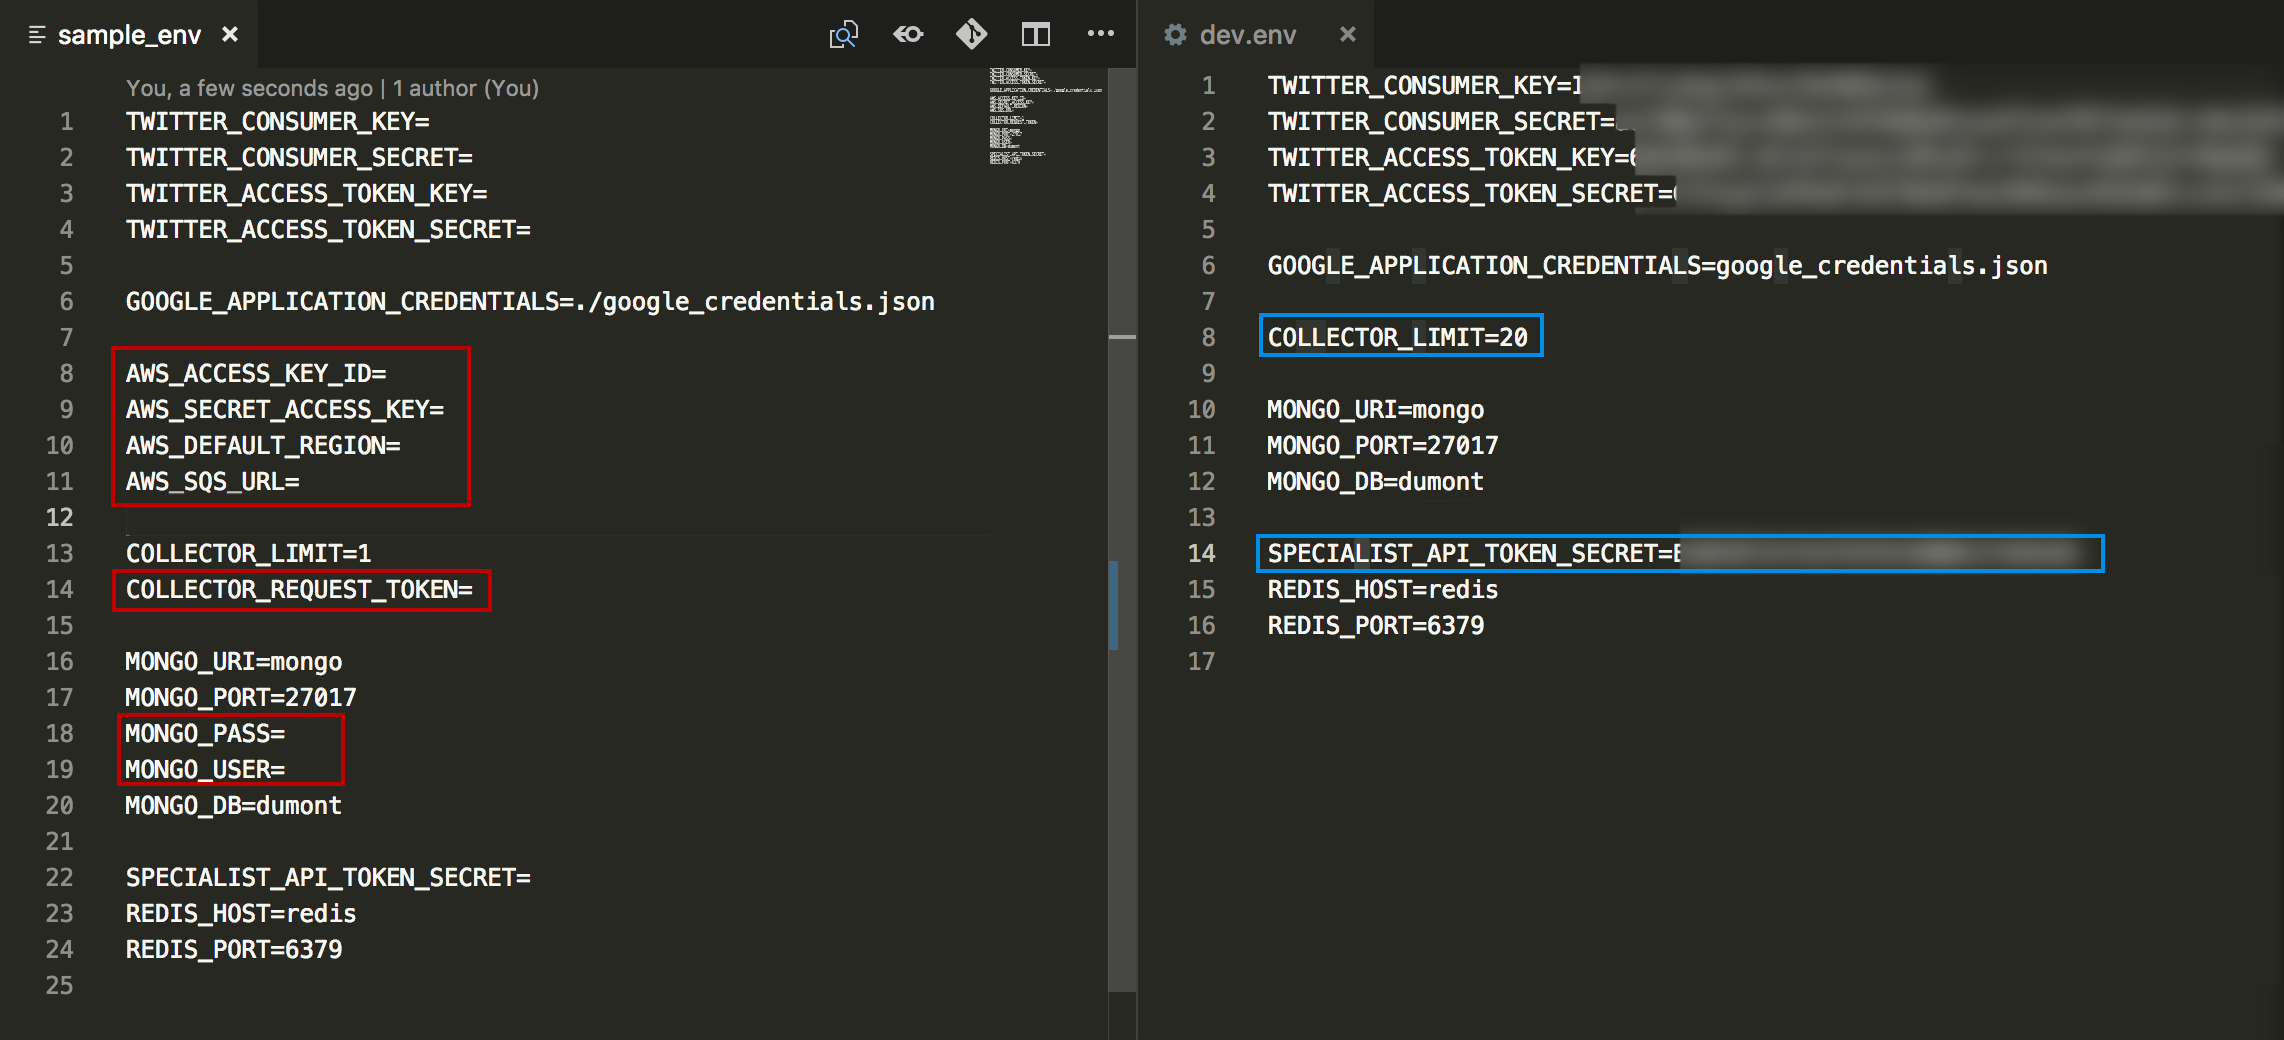
\includegraphics[width=1\textwidth]{imagens/creds.png}
    \caption{Imagem demonstrando passo a passo de como gerar o JSON de credencial}
    \label{fig:creds}
\end{figure}

É importante lembrar dos limites da API publica do twitter, e tambem que devido a implementação (que pode ser acompanhada no arquivo \textit{dumont/collector/twitter/index.js}) na linha 74 é possível ver o momento onde a \textit{stream} é parada, entretando, podem chegar inumeros tweets de diferentes usuarios simuntaneamente, fazendo assim, com que sobrecarregue a quantiadade de usuarios permitidas na API. É sugerido rodar valores baixos entre 20 a 45 para evitar problemas.

Uma vez configurado, é possivel executar o comando \textit{docker-compose -f docker-compose.dev.yml}, uma vez que o docker inicie o serviço você pode iniciar a coleta utilizando desde um navegador, ferramentas (um exemplo é o Postman\footnote{https://www.getpostman.com/}) ou até mesmo o \textit{curl} utilizando o uri \textit{\url{http://127.0.0.1:8080/}}

Depois que os dados foram coletados, ja é possível minerar algumas informações deles, para isso existem processos a serem detalhados.
